\section{Примеры работы программы}

\subsection{Описание программного решения}

Для решения задачи в среде \textit{MatLab} были написаны функции для каждого требуемого Разделом~1 пункта постановки задачи. Взаимодействие с данными функциями реализуется при помощи интерфейса глобальных переменных, которые принимают условие задачи, а также содержат другие общие для \textit{программного решения} данные. Для удобства использования программного решения реализован графический интерфейс для наиболее часто употребимых функций.

\begin{figure}[h]
\noindent\centering{
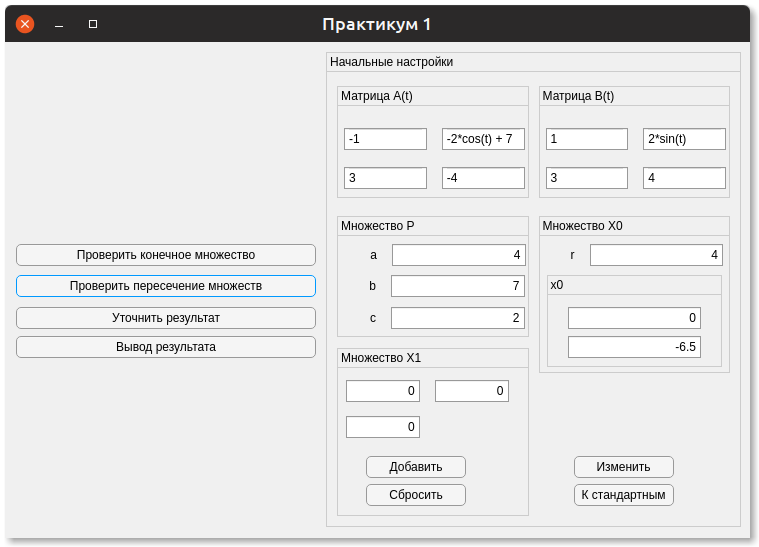
\includegraphics[width=120mm]{program/app.png}
}
\caption{Графический интерфейс программы.}
\label{img:app}
\end{figure}

Далее рассмотрим результаты численного решения задачи для разных начальных данных. Для того, чтобы отличие было более наглядным, зафиксируем начальное, целевое и ограничивающее множества в положении
$$
        B(t) =
        \begin{pmatrix}
                1 & 2\sin t\\
                3 & 4
        \end{pmatrix}, 
$$
$$
        a = 4,\quad b = 7,\quad c = 2,
$$
$$
        x_0 = (-3,\,-7)^\T,\quad r = 4,
$$
$$
        G =
        \begin{pmatrix}
                \;\;\;0{,}3 & \;\;4\\
                -0{,}4 & -2 \\
                \;\;\;0{,}2 & -2
        \end{pmatrix},
        \quad g =
        \begin{pmatrix}
                -10 \\
                \;\;-3 \\
                \;\;-4
        \end{pmatrix}
$$
и обратим внимание на различия численного решения при разных матрицах $A(t)$. Для простоты будем брать константные матрицы $A(t) \equiv A$ с различным типом собственных значений.


\subsection{$A$ с вещественными собственными значениями}

Рассмотрим фазовый портрет, ,,оптимальное‘‘ управление и ,,оптимальную‘‘ траекторию, построенные программой для матрицы
$$
        A =
        \begin{pmatrix}
        1 & 1 \\
        2 & -7 \\
        \end{pmatrix}.
$$
\begin{figure}[h]
\noindent\centering{
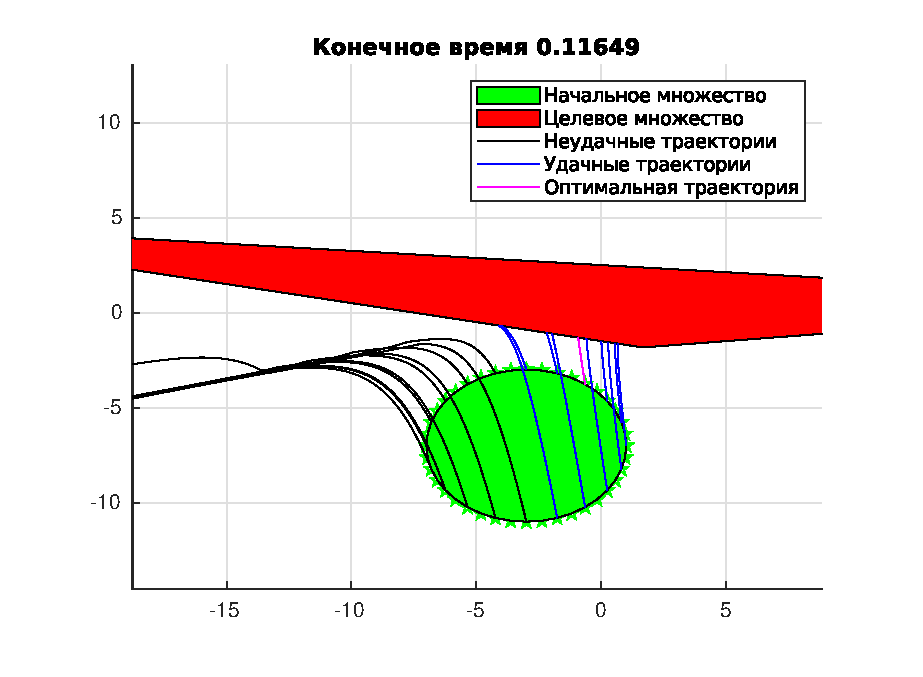
\includegraphics[width=120mm]{program/real-tr.eps}
}
\caption{Фазовый портрет задачи \eqref{eq:main_system} при вещественных собственных значениях матрицы $A$.}
\end{figure}

\begin{figure}[h]
                \hfill
                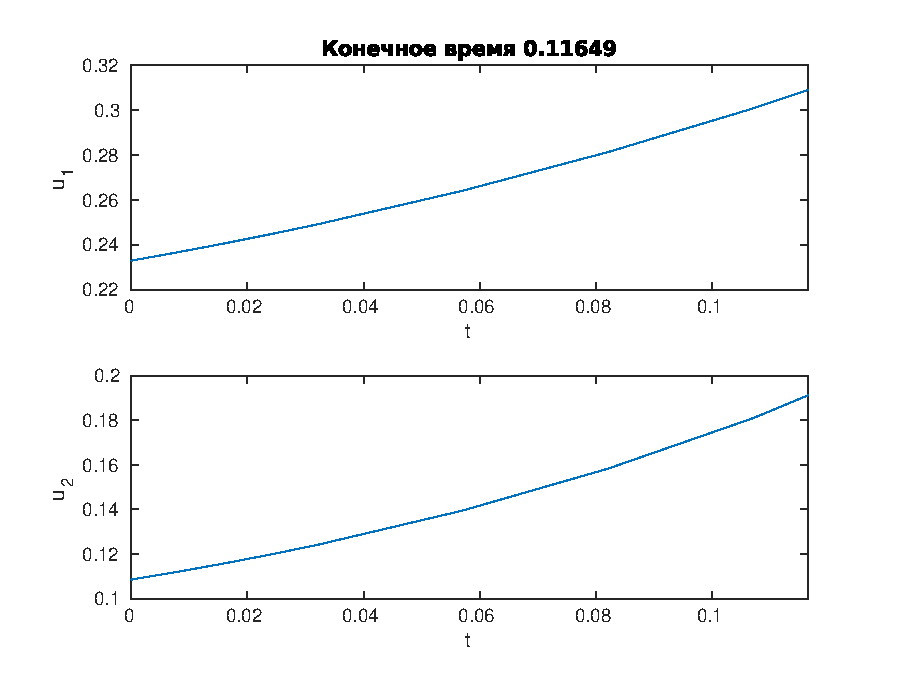
\includegraphics[width=70mm]{program/real-control.eps}
                \hfill
                \hfill
                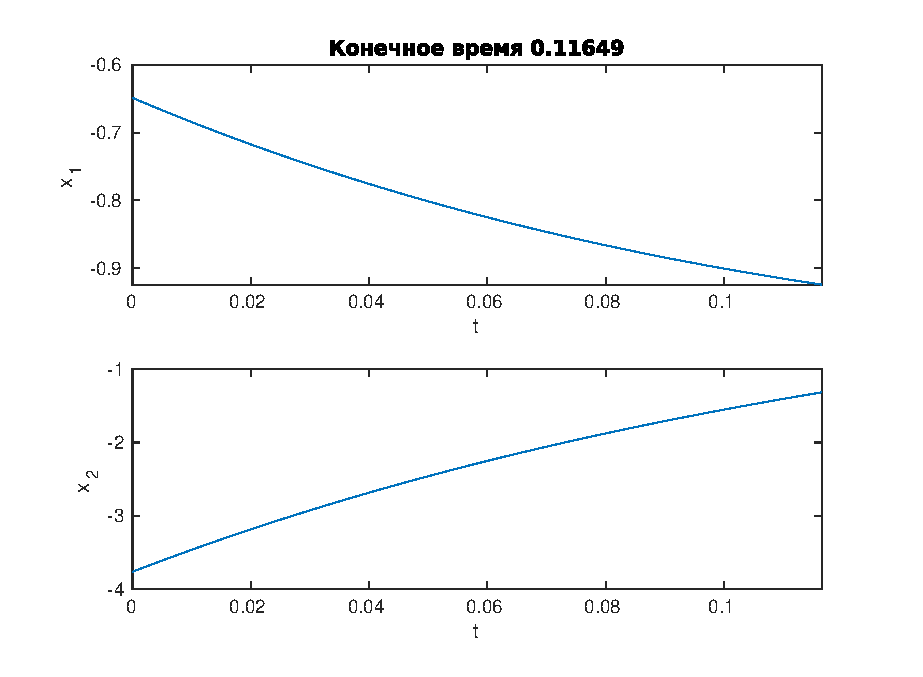
\includegraphics[width=70mm]{program/real-traectory.eps}
                \hfill
                \caption{,,Оптимальное‘‘ управление и ,,оптимальная‘‘ интегральная кривая задачи \eqref{eq:main_system} при вещественных собственных значениях матрицы $A$.}
\end{figure}

\subsection{$A$ с комплексными собственными значениями}

Рассмотрим фазовый портрет, ,,оптимальное‘‘ управление и ,,оптимальную‘‘ траекторию, построенные программой для матрицы
$$
        A =
        \begin{pmatrix}
        -9 & -10 \\
        21 & -7 \\
        \end{pmatrix}.
$$
\begin{figure}[h]
\noindent\centering{
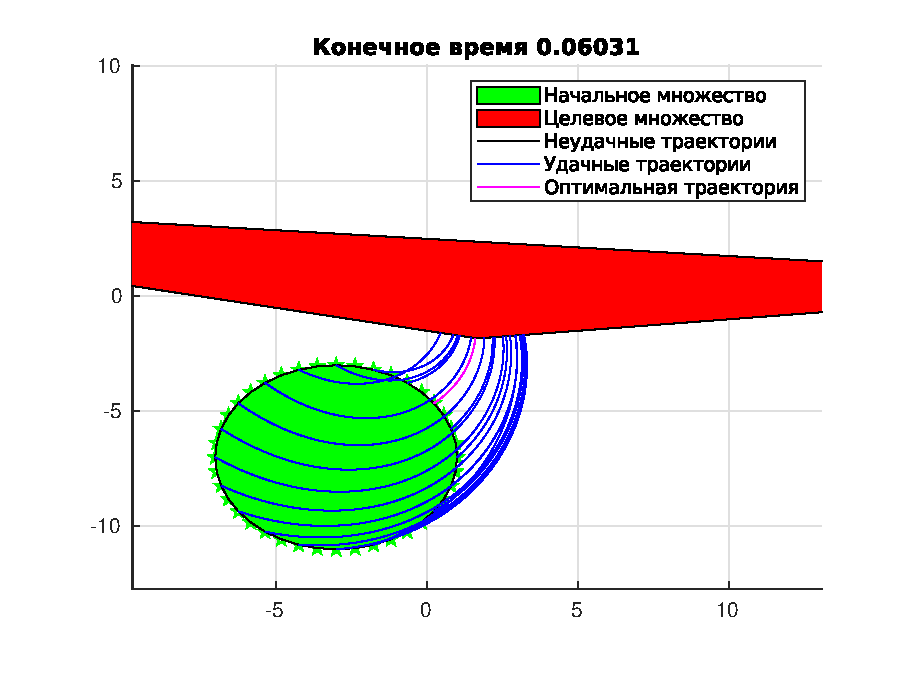
\includegraphics[width=120mm]{program/complex-tr.eps}
}
\caption{Фазовый портрет задачи \eqref{eq:main_system} при комплексных собственных значениях матрицы $A$.}
\end{figure}

\begin{figure}[h]
                \hfill
                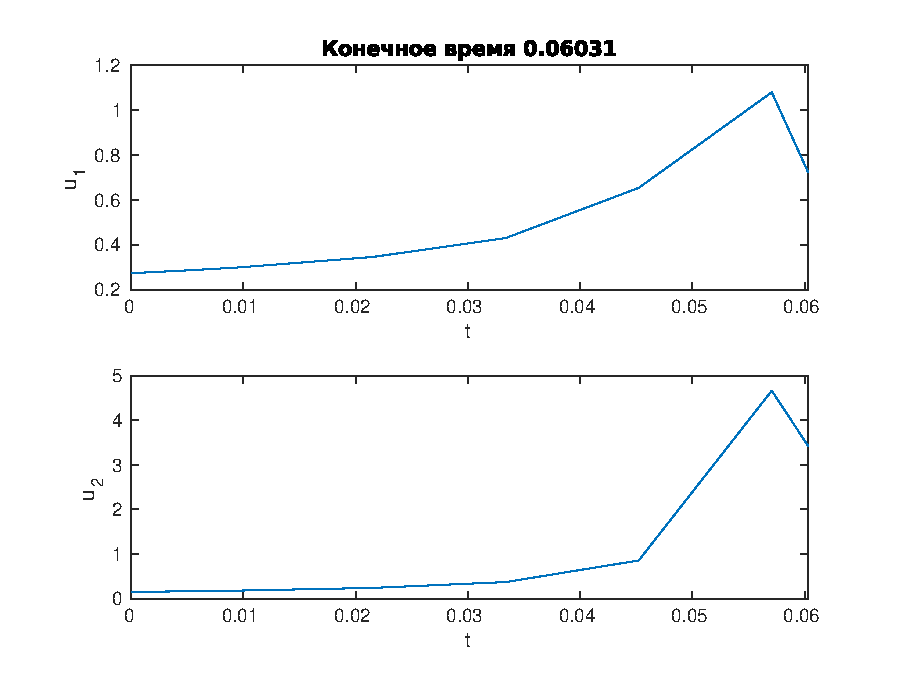
\includegraphics[width=70mm]{program/complex-control.eps}
                \hfill
                \hfill
                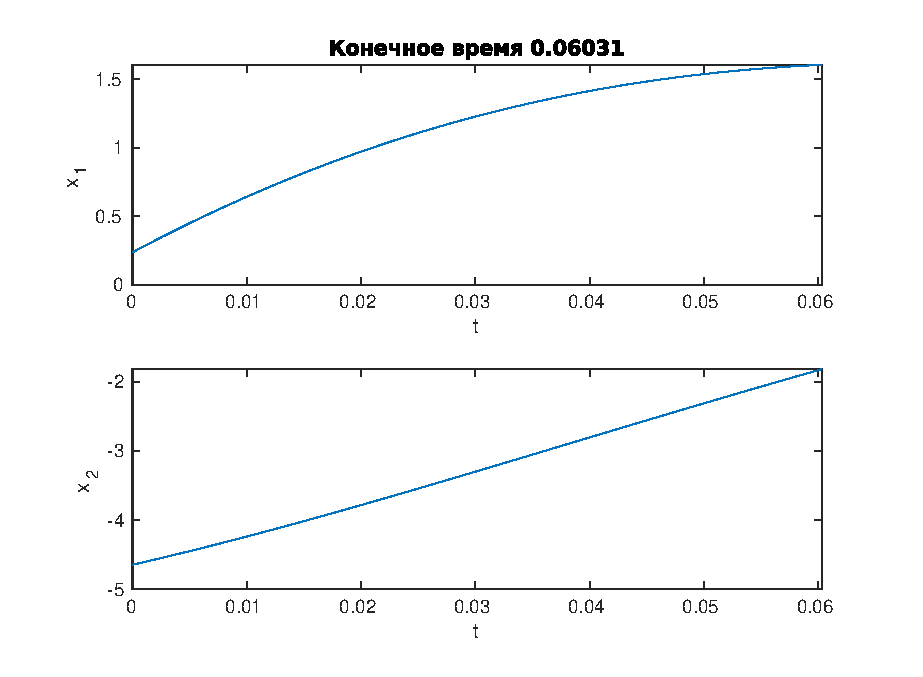
\includegraphics[width=70mm]{program/complex-traectory.eps}
                \hfill
                \caption{,,Оптимальное‘‘ управление и ,,оптимальная‘‘ интегральная кривая задачи \eqref{eq:main_system} при комплексных собственных значениях матрицы $A$.}
\end{figure}

\subsection{$A$ вырождена}

Рассмотрим фазовый портрет, ,,оптимальное‘‘ управление и ,,оптимальную‘‘ траекторию, построенные программой для матрицы
$$
        A =
        \begin{pmatrix}
        -1 & -1 \\
        -1 & -1 \\
        \end{pmatrix}.
$$
\begin{figure}[h]
\noindent\centering{
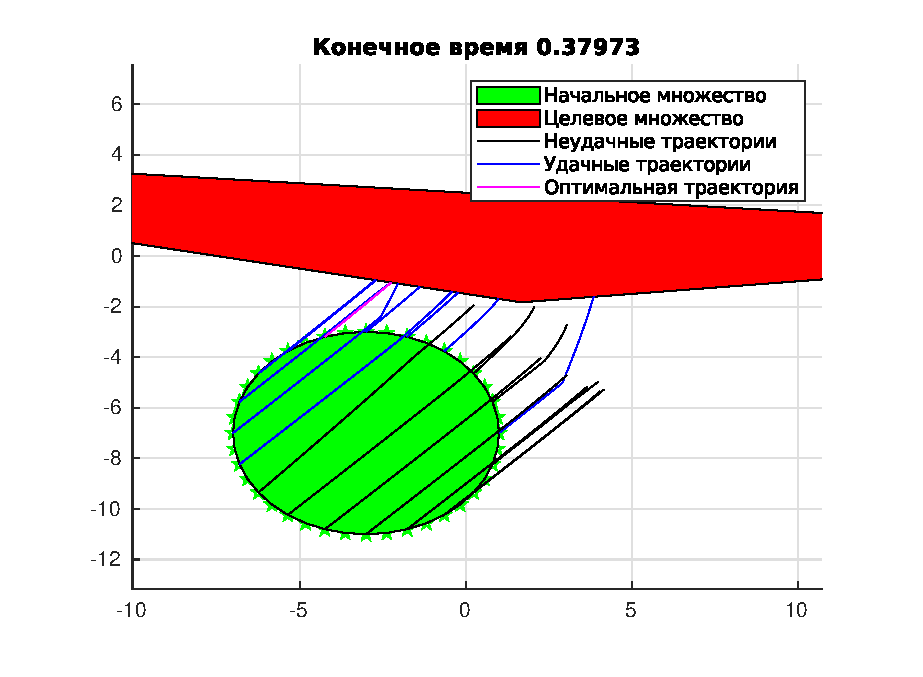
\includegraphics[width=120mm]{program/v-tr.eps}
}
\caption{Фазовый портрет задачи \eqref{eq:main_system} при вырожденной матрице $A$.}
\end{figure}

\begin{figure}[h]
                \hfill
                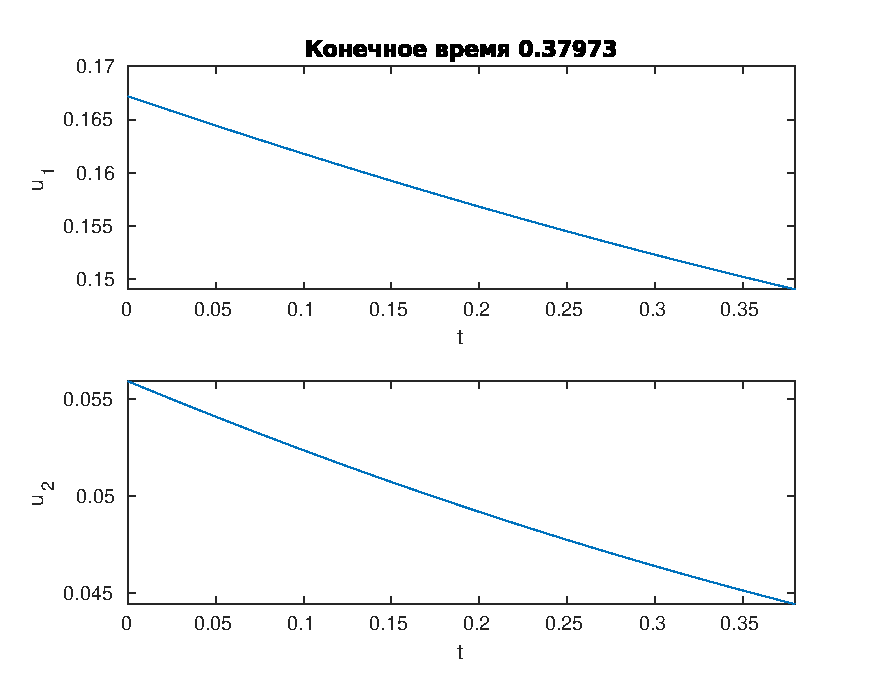
\includegraphics[width=70mm]{program/v-control.eps}
                \hfill
                \hfill
                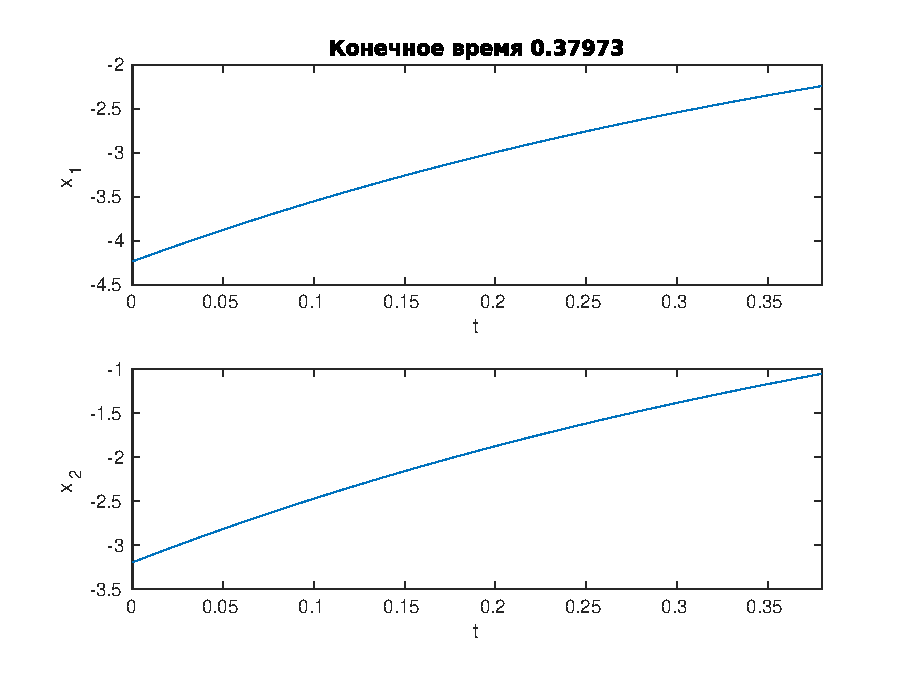
\includegraphics[width=70mm]{program/v-traectory.eps}
                \hfill
                \caption{,,Оптимальное‘‘ управление и ,,оптимальная‘‘ интегральная кривая задачи \eqref{eq:main_system} при вырожденной матрице $A$.}
\end{figure}


\subsection{Отсутствие непрерывной зависимости времени быстродействия от параметров системы}

Рассмотрим задачу \eqref{eq:main_system} со следующими параметрами:
$$
        A = \begin{pmatrix} 1 & 4 \\ -4 & 1 \end{pmatrix}, \quad
        B = \begin{pmatrix} 1 & 2\sin t \\ 3 & 4 \end{pmatrix},
$$
$$
        a = 4,\,b=7,\,c=2,\,r=4,\,x_0 = [0,\,10]^\T.
$$
Целевое множество $\X_1$ \textit{немного изменим}, то есть построим ,,оптимальные‘‘ траектории для параметров:
$$
        G_1 = \begin{pmatrix}
        \;\;\;0{,}3 & \;\;4\\
        -0{,}4 & -2 \\
        \;\;\;0{,}2 & -2 \\
        \;\;\;\;\;\;1 & \;\;\;0
        \end{pmatrix},\;
        g_1 = \begin{pmatrix}
                \;-10 \\
                \;\;\;-3 \\
                \;\;\;-4 \\
                -8{,}7
        \end{pmatrix}
        \quad
        \mbox{и}
        \quad
        G_2 = \begin{pmatrix}
        \;\;\;0{,}3 & \;\;4\\
        -0{,}4 & -2 \\
        \;\;\;0{,}2 & -2 \\
        \;\;\;\;\;\;1 & \;\;\;0
        \end{pmatrix},\;
        g_2 = \begin{pmatrix}
                \;-10 \\
                \;\;\;-3 \\
                \;\;\;-4 \\
                -8{,}6
        \end{pmatrix}.
        $$
Эти параметры на $0{,}1$ сдвигают правую границу целевого множества $\X_1$ (см. Рис.~\ref{img:change_finish_set}).

\begin{figure}[h]
                \hfill
                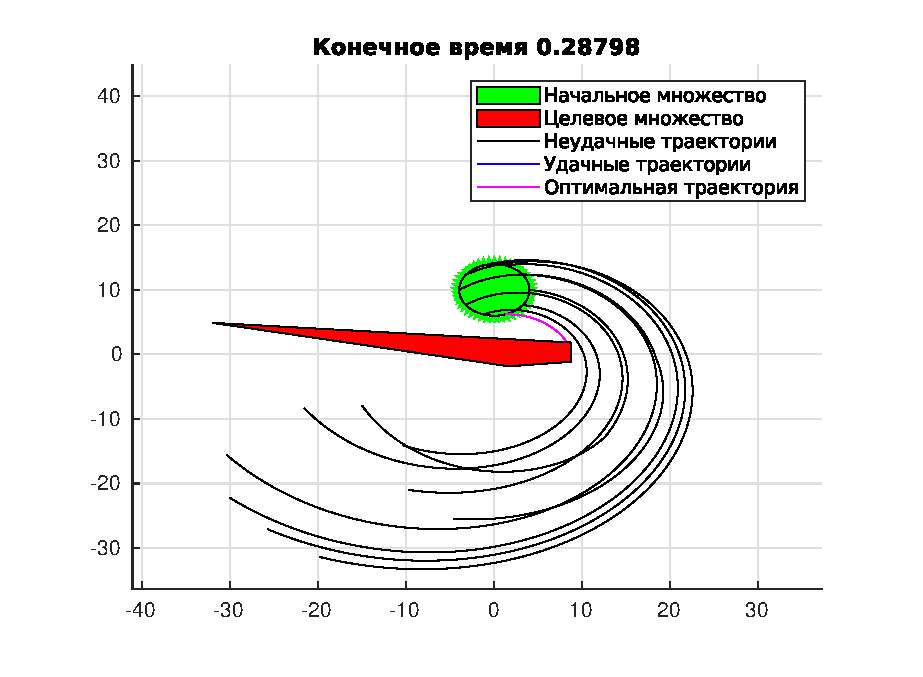
\includegraphics[width=70mm]{program/t8n7.eps}
                \hfill
                \hfill
                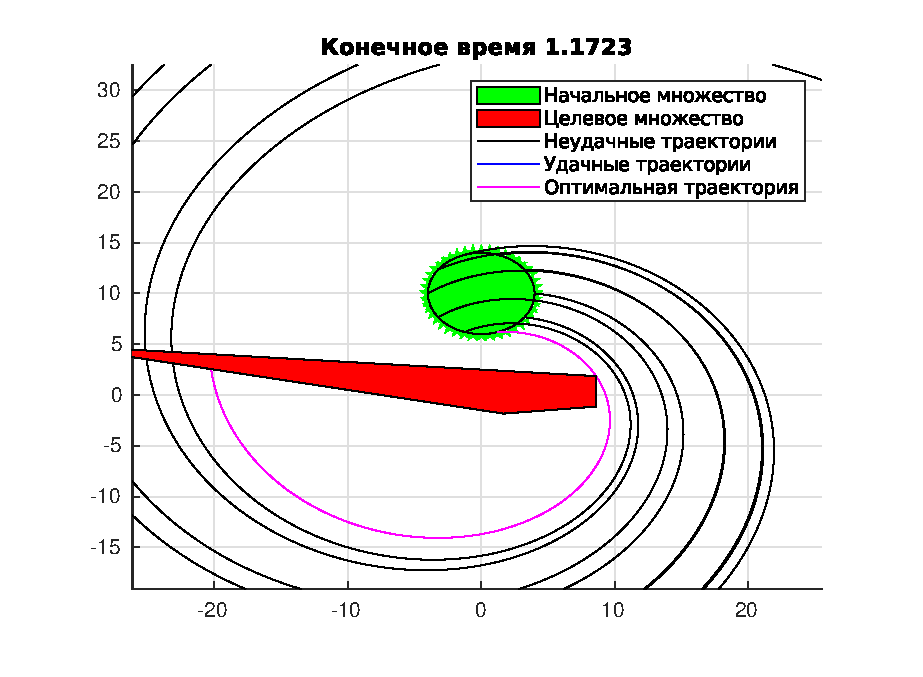
\includegraphics[width=70mm]{program/t8n6.eps}
                \hfill
                \caption{\textit{Небольшое изменение} целевого множества.}
                \label{img:change_finish_set}
\end{figure}

Отчётливо видно, что при достаточно малом изменении целевого множества время быстродействие увеличилось на $0{,}88$, так как ,,оптимальная‘‘ траектрория для первых параметров стала обходить угол целевого множества~$\X_1$. Этот пример демонстрирует отсутствие непрерывной зависимости времени быстродействия от парамеров задачи~\eqref{eq:main_system}.